\chapter{Wstęp teoretyczny}
\label{cha:wstep}

% Informacje teoretyczne o wykorzystanych narzędziach, technologiach itp..
% tu generalne wprowadzenie do tematu

Rozdział zawiera podstawowe informacje teoretyczne niezbędne do zrozumienia opisywanych w~pracy zagadnień. Wyjaśniono kluczowe pojęcia używane w~tekście oraz przedstawiono metody wykorzystane w~części praktycznej projektu. 

%---------------------------------------------------------------------------

\section{Kamery zdarzeniowe}
\label{sec:kamery_zdarzeniowe}

% Budowa i działanie, dane event frame'y, jakieś grafiki
Kamery zdarzeniowe (ang. \textit{Dynamic Vision Sensors (DVS)}) to urządzenia rejestrujące obraz w~sposób odmienny od tradycyjnych kamer klatkowych, które zapisują obrazy w~regularnych odstępach czasu (np. 30 klatek na sekundę). W~odróżnieniu od nich, kamery zdarzeniowe rejestrują jedynie zmiany jasności w~poszczególnych pikselach matrycy. Porównanie sposobu, w~jaki rejestrowane są dane w~kamerze tradycyjnej i~zdarzeniowej, przedstawione jest na rysunku \ref{fig:dvs_vs_camera}. Wyjście zwykłej kamery to klatki, pojawiające się co pewien stały czas i~zawierające pełny widok, podczas gdy jedynym obiektem pojawiającym się na wyjściu DVS jest poruszający się obiekt, rejestrowany jako osobne, często występujące asynchroniczne zdarzenia.

Każdy piksel DVS działa niezależnie i~rejestruje zdarzenie w momencie, gdy różnica jasności padającego na nie światła przekroczy określony próg. 

Szczegółowe informacje na temat działania i~sposobów wykorzystania tych kamer można znaleźć w~artykule \cite{dvs_survey}.

\begin{figure}
    \centering
    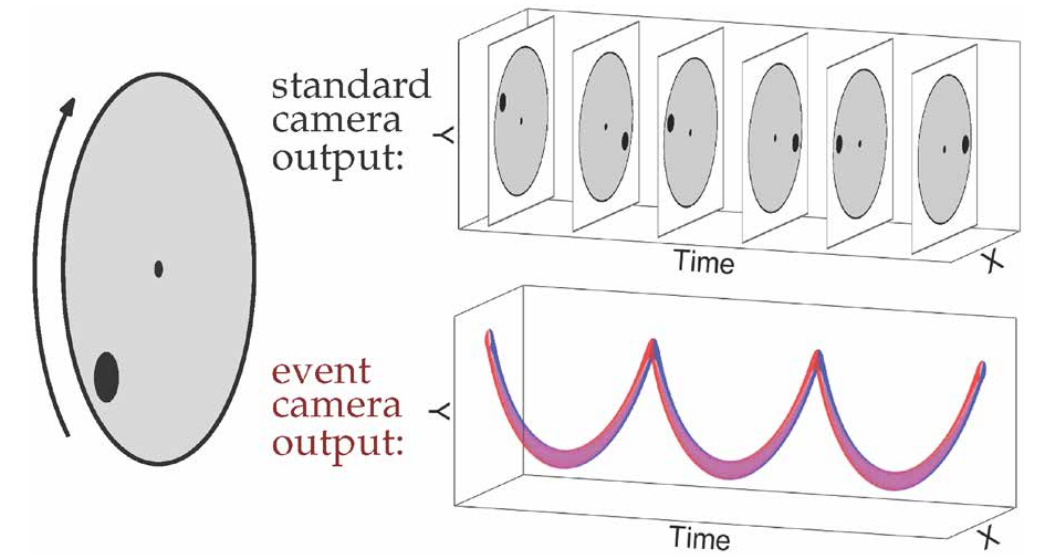
\includegraphics[width=0.7\linewidth]{images/events_dynamic_obstacle.png}
    \caption{Porównanie sposobu rejestracji danych przez zwykłą kamerę i~DVS.}
    \label{fig:dvs_vs_camera}
\end{figure}

Kamera zdarzeniowa podaje na wyjście asynchroniczny strumień zdarzeń (ang. \textit{event}), z~których każdy jest krotką w formacie: $$(t, x, y, p)$$ 
gdzie:

$t$ -- czas wystąpienia zdarzenia (ang. \textit{timestamp}),

$x$, $y$ -- położenie piksela w matrycy,

$p$ -- polaryzacja zdarzenia (ang. \textit{polarity}) -- mówi o~kierunku zmiany jasności piksela, przyjmuje wartości $-1$ lub $1$ (czasami przyjmuje się wartości $0$ oraz $1$).
\vspace{11px}

W celu wizualizacji zdarzeń na płaszczyźnie obrazu stosuje się metody ich reprezentacji w~postaci tzw. \textit{event frame}'ów, czyli pewnego rodzaju klatek zdarzeniowych. Istnieje kilka podejść, ale w~tym projekcie są one tworzone przy wykorzystaniu reprezentacji \textit{exponentially decaying time surface} \cite{Blachut_2023}. W metodzie tej wartość piksela na obrazie obliczana jest na podstawie jego \textit{timestampu}, przy zastosowaniu funkcji (\ref{agreg}). Dzięki temu jasność piksela na obrazie wskazuje na to, jak dawno wystąpiło tam zdarzenie. 

\begin{align}
    f(t, u) = p_u * e^{\frac{t_u - t}{\tau}} \label{agreg}
\end{align}

\noindent gdzie:
\begin{itemize}
    \item $u, p_u, t_u$ -- odpowiednio: zdarzenie, jego polaryzacja i~czas wystąpienia,
    \item$f(t, u)$ -- wartość jasności piksela na \textit{event frame}'ie,
    \item $\tau$ -- czas, który obejmuje klatka, czyli różnica czasu wystąpienia najstarszego i~najmłodszego zdarzenia.
\end{itemize}


% działanie pojedyńczego piksela???

% Szum i jego rodzaje leakage, shot i thermal noise???

% Zalety - lista, Rola w projekcie

DVS pozbawione są ograniczeń związanych z~rejestracją danych ze stosunkowo niewielką częstotliwością -- tradycyjne kamery odczytują obraz z częstotliwością kilkudziesięciu Hz, natomiast kamery zdarzeniowe działają z~minimalnym opóźnieniem, sięgającym mikrosekund (np. dla DAVIS346 -- ok. \SI{12}{\micro\Hz}), czyli teoretyczna częstotliwość odczytu zdarzeń sięga dziesiątek kHz. Efektem takiego sposobu działania jest niska latencja.
Dzięki rejestracji wyłącznie pojedynczych zdarzeń zamiast całych klatek (brak redundancji danych), kamery zdarzeniowe pozwalają na oszczędzanie pamięci i~energii. Efekt ten jest szczególnie wyraźny w przypadku statycznych scen, w~których pojawia się niewiele ruchomych obiektów. Kolejną zaletą jest wysoka odporność na występowanie zmiennego oświetlenia, dzięki szerokiej rozpiętości tonalnej (ang. \textit{high dynamic range}), osiągniętej dzięki asynchroniczności i~niezależności działania pikseli.

Ograniczeniem DVS jest wrażliwość na występowanie szumu, czyli pojawianie się na wyjściu fałszywych zdarzeń. Kolejną wadą jest nietypowy format danych wyjściowych, który uniemożliwia bezpośrednie wykorzystanie do ich przetwarzania algorytmów stosowanych dla zwykłych kamer. Warto również wspomnieć o~ograniczonych możliwościach dostarczania informacji o~statycznych scenach, gdy ruch nie występuje lub jest bardzo powolny. Koszt zakupu kamery zdarzeniowej znacznie przewyższa cenę tradycyjnej kamery.

\section{Robot Operating System (ROS)}

% Wprowadzenie

\textbf{ROS2} (ang. \textit{Robot Operating System 2}) to otwartoźródłowy \textit{framework}, który ułatwia projektowanie, rozwój i~wdrażanie systemów robotyki. Jest platformą programistyczną zapewniającą zestaw gotowych funkcji, bibliotek i~narzędzi wspomagających komunikację, percepcję, sterowanie oraz współpracę robotów. ROS2 można traktować jako ,,warstwę pośrednią'', która zarządza wymianą informacji między różnymi elementami robota. Jego głównym zadaniem jest zapewnienie płynnego przepływu danych między tymi elementami i~umożliwienie ich współpracy.
ROS2 wspiera języki programowania C++ oraz Python. W~projekcie wykorzystany został ten drugi.

Działanie ROS-a bazuje na równolegle pracujących i~asynchronicznie komunikujących się węzłach (ang. \textit{nodes}), czyli jednostkach wykonawczych, które realizują konkretne zadania w systemie. Każdy węzeł działa jako niezależny proces i~może komunikować się z~innymi węzłami. Podstawowy sposób komunikacji to \textit{topic}, który jest kanałem komunikacyjnym, na którym węzły mogą publikować dane lub je subskrybować, umożliwiając asynchroniczną wymianę informacji. Dane przesyłane przez \textit{topic} mają postać wiadomości (ang. \textit{messages}), które posiadają predefiniowany typ, np. dane obrazu, pozycja robota czy informacje tekstowe. Dzięki tej architekturze węzły mogą niezależnie wymieniać informacje, co zapewnia modułowość i~elastyczność systemu.

Przykład działania:
\begin{itemize}
    \item Węzeł A (np. kamera) \textbf{publikuje} (czyli regularnie nadaje do węzłów odbierających (ang. \textit{subscriber})) dane obrazu na \textit{topic} -- na przykład \textit{/camera/image\_raw},
    \item Węzeł B (np. algorytm przetwarzania obrazu) \textbf{subskrybuje} ten sam \textit{topic}, aby odbierać dane,
    \item Dane (wiadomości) zaczynają być przesyłane z~węzła A do węzła B.
\end{itemize}
    
Inne sposoby na komunikację między węzłami to:
\begin{itemize}
    \item usługi (ang. \textit{services}) -- pozwalają na dwustronną komunikację, w~której jeden węzeł wysyła żądanie i~otrzymuje od drugiego odpowiedź,
    \item akcje (ang. \textit{actions}) -- pozwalają na wykonywanie zadań długotrwałych, gdzie węzeł może otrzymywać aktualizacje postępu i~anulować zadanie w~trakcie jego realizacji.
\end{itemize}


% ROS1 a ROS2


\section{Testowanie systemów wbudowanych}
\label{sec:testowanie_teoria}

W~procesie rozwoju systemów oprogramowania i~algorytmów dla systemów wbudowanych, ważna jest możliwość testowania i~oceny działania na wszystkich etapach pracy. W~zależności od stopnia postępów, wykorzystuje się w~tym celu różne metody.

% Wprowadzenie
\subsection{Software in the Loop}
% Co to SiL, dlaczego się je tworzy i wykorzystuje
\textit{Software in the Loop} (SiL) to metoda testowania stosowana na wczesnym etapie rozwijania systemu wbudowanego. W procesie SiL cały system jest uruchamiany w środowisku komputerowym, gdzie wszystkie fizyczne komponenty są symulowane, np. przy użyciu wirtualnych czujników, silników czy urządzeń wejścia/wyjścia. Następnie algorytmy sterowania, przetwarzania danych czy komunikacji są testowane w~tym wirtualnym środowisku, co pozwala na wczesne wykrycie błędów i~optymalizację oprogramowania przed przejściem do bardziej kosztownych etapów testów.

Zalety metody \textit{Software in the Loop} to:
\begin{itemize}
    \item Skrócenie czasu testowania -- umożliwia szybkie testowanie i~weryfikację algorytmów bez potrzeby korzystania z~fizycznych komponentów, co przyspiesza proces rozwoju,
    \item Niskie koszty -- testowanie w~środowisku symulacyjnym eliminuje koszty związane z~wykorzystaniem sprzętu oraz ryzyko jego uszkodzenia podczas testów,
    \item Bezpieczeństwo -- pozwala na testowanie potencjalnie niebezpiecznych scenariuszy bez ryzyka uszkodzenia rzeczywistych urządzeń lub zagrożenia dla ludzi,
    \item Łatwość w~modyfikacjach -- symulowane środowisko pozwala na łatwe wprowadzanie zmian,
    \item Szybka identyfikacja błędów -- umożliwia szybkie wykrycie problemów w~kodzie.
\end{itemize}


% Wykorzystanie w projekcie - Co to Gazebo i jakie nam daje możliwości - jest opisane niżej




\subsection{Hardware in the Loop}
\label{subsec:hil}

% Opis metody HIL

\textit{Hardware in the Loop} (HiL) to metoda testowania, w~której rzeczywisty sprzęt jest połączony z~symulowanym środowiskiem, co pozwala na weryfikację działania systemu na docelowej platformie obliczeniowej. W~tej metodzie część systemu jest symulowana komputerowo (dynamika obiektów, emulacja czujników), a~część działa na rzeczywistym sprzęcie. Dzięki temu można testować interakcje między sprzętem a~oprogramowaniem, co umożliwia dokładne sprawdzenie działania systemu przed jego pełnym wdrożeniem.

HiL pozwala na realistyczne testowanie algorytmów sterowania i~interakcji między różnymi elementami systemu, bez potrzeby uruchamiania pełnego prototypu w~rzeczywistych. To podejście zapewnia większe bezpieczeństwo i~zmniejsza ryzyko uszkodzenia sprzętu, ponieważ testy mogą odbywać się w~kontrolowanym środowisku. Ponadto umożliwia optymalizację algorytmów i~dokładną walidację działania systemu.

Przewaga nad SiL polega na możliwości sprawdzenia działania oprogramowania na docelowym sprzęcie -- warunki są więc bardziej zbliżone do rzeczywistych.

% Dlaczego ten sposób testowania? - co się zyskuje względem SiL?




\section{Triangulacja jako metoda estymacji głębi}
\begin{figure}
    \centering
    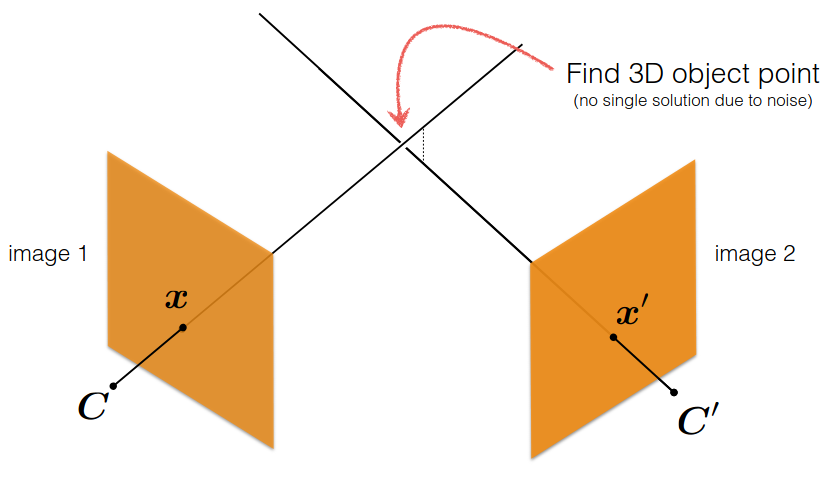
\includegraphics[width=0.8\linewidth]{images/triangulation.png}
    \caption{Idea triangulacji. $C$ i~$C'$ to punkty centralne na matrycach kamer. $x$ i~$x'$ to położenia tego samego obiektu (punktu w przestrzeni 3D) na płaszczyznach obrazu. Długość odcinka między punktami $C$ i~$x$ jest określona przez ogniskowe kamer. W~idealnym przypadku (brak szumu, dokładnie ten sam czas rejestracji obu klatek) półproste będące przedłużeniem tych odcinków powinny przeciąć się jednym punkcie -- rozwiązaniu. Źródło: \cite{triangulation}.}
    \label{fig:triangulation}
\end{figure}

% Parametry zewnętrzne i wewnętrzne kamer
Aby przeprowadzić estymację głębi punktu widocznego na obrazie z dwóch kamer, w pierwszej kolejności konieczne jest odczytanie ich parametrów. Dostarczają one informacji na temat położenia kamery w przestrzeni oraz o sposobie przekształcania trójwymiarowych punktów świata rzeczywistego na dwuwymiarowy obraz.

\vspace{11px}
\noindent Parametry wewnętrzne:

\begin{itemize}
    \item macierz $K$ (\ref{K_matrix}) -- macierz, która zawiera informacje o~parametrach wewnętrznych takich jak: ogniskowa dla osi x -- $f_x$ oraz y -- $f_y$ i~współrzędne punktu głównego (centrum obrazu) -- $c_x$ i~$c_y$,
    \begin{align}
        K = \begin{bmatrix} \label{K_matrix}
        f_x & 0 & c_x \\
        0 & f_y & c_y \\
        0 & 0 & 1
        \end{bmatrix}
    \end{align}
    \item wektor dystorsji (\ref{dist}) -- opisuje zniekształcenie obrazu. Współczynniki $k$ to wartość dystorsji radialnej, a~$p$ -- tangencjalnej. Jeżeli wektor ten nie jest zerowy, to należy użyć go do korekcji zniekształceń obrazu.
    \begin{align}
        d = \begin{bmatrix} \label{dist}
        k_1 & k_2 & k_3 & p_1 & p_2
        \end{bmatrix}
    \end{align}
\end{itemize}

\noindent Parametry zewnętrzne:

\begin{itemize}
    \item translacja (\ref{trans}) -- położenie kamery w~przestrzeni 3D,
    \begin{align}
        t = \begin{bmatrix} \label{trans}
        x \\ y \\ z
        \end{bmatrix}
    \end{align}
    \item orientacja -- zwykle w~formie macierzy $R$ o~rozmiarze $3 \times 3$. Dostarcza informacji o~rotacji kamery.
\end{itemize}

Zasada triangulacji przedstawiona jest na rysunku \ref{fig:triangulation}. Należy znaleźć współrzędne punktu przecięcia półprostych poprowadzonych przez punkty $C$ i~$x$ obu kamer. W~tym celu należy wyznaczyć ich macierze projekcji (\ref{proj}), które łączą parametry zewnętrzne i~wewnętrzne.

\begin{align}
    P = K \cdot [R | t] \label{proj}
\end{align}

Macierzy projekcji można użyć do sformułowania równań, w~których niewiadomymi będą współrzędne poszukiwanego punktu $\mathbf{X}$.

\begin{align}
    P \cdot \mathbf{X} = x, \quad P' \cdot \mathbf{X} = x' \label{eqations}
\end{align}

\noindent gdzie:

$P$ i $P'$, to macierze projekcji odpowiednio pierwszej i~drugiej kamery -- wartości znane,

$\mathbf{X}$ to wektor współrzędnych szukanego punktu w~trójwymiarowej przestrzeni,

$x$ i $x'$ to położenie obrazu obiektu na płaszczyznach kamer w~przestrzeni 3D -- wartości znane.

\vspace{11px}
Pojedyncze równanie z (\ref{eqations}) można zapisać jako:
\begin{align}
    \begin{bmatrix}
        p_{11} & p_{12} & p_{13} & p_{14} \\
        p_{21} & p_{22} & p_{23} & p_{24} \\
        p_{31} & p_{32} & p_{33} & p_{34}
\end{bmatrix} \cdot 
\begin{bmatrix}
    X_0 \\
    Y_0 \\
    Z_0 \\
    1
\end{bmatrix} = 
\begin{bmatrix}
    x_0 \\
    y_0 \\
    z_0
\end{bmatrix}
\end{align}

Współrzędne punktów $x$ i~$x'$ można otrzymać przez przekształcenie ich współrzędnych z~obrazu do przestrzeni kamery za pomocą równania (\ref{2d3d}).

\begin{align}
    \begin{bmatrix} x_0 \\ y_0 \\ z_0 \end{bmatrix} = K^{-1} \cdot \begin{bmatrix} u \\ v \\ 1 \end{bmatrix} \label{2d3d}
\end{align}

\noindent gdzie:

$u$ i~$v$ to współrzędne obiektu na obrazie.
\vspace{11px}

W celu wyznaczenia głębi, trzeba znaleźć rozwiązanie najlepiej spełniające równania (\ref{eqations}). Jednoznaczne rozwiązanie prawdopodobnie nie istnieje z~uwagi na niedokładności wynikające chociażby z~powodu występowania szumu.

Jeżeli układem odniesienia w~trójwymiarowej przestrzeni, w~jakim rozpatrywane były wszystkie współrzędne punktów, była jedna z~kamer, to odległość do niej jest równa współrzędnej $Z_0$ wynikowego wektora $\mathbf{X}$.

\vspace{11px}

Układ stereo kamer oznacza dwie kamery skonfigurowane do wspólnej pracy w celu estymacji głębi. Często umieszczone są one w~jednej obudowie w~taki sposób, by zachowywały te same parametry (z~wyjątkiem translacji). Oznacza to, że przekształcają one punkty z przestrzeni 3D na płaszczyznę obrazu w~ten sam sposób i~nie są obrócone względem siebie. Pozwala to na uproszczenie obliczeń.

\section{Platformy sprzętowe}
% Opisuję bardzo krótko, bo i tak nie użyłem

Aby zintegrować system wbudowany na rzeczywistym dronie lub robocie mobilnym, należy zaimplementować go na wbudowanej platformie obliczeniowej, która zapewni możliwość działania oprogramowania.

W~celu implementacji systemów wizyjnych, często stosowana platforma -- mikrokontroler, wyposażony w~mikroprocesor, może okazać się nieodpowiednim rozwiązaniem. Powodem tego jest duża ilość danych przetwarzana przez algorytmy wizyjne. Szczególnie kiedy wymagane jest niezawodne działanie systemu w~czasie rzeczywistym, należy skorzystać z innych platform obliczeniowych, które pozwalają na zrównoleglenie obliczeń i~w~konsekwencji przyśpieszą czas ich wykonywania.

\vspace{11px}

Pierwszym rozwiązaniem jest zastosowanie układu SoC (ang. \textit{System on Chip}) z~wbudowanym procesorem graficznym (ang. \textit{Graphics Processing Unit (GPU)}). Takim układem jest płytka z serii eGPU Jetson. SoC oznacza układ zawierający kompletny system elektroniczny -- w~tym przypadku mikrokontroler, GPU i~peryferia. Takie rozwiązanie pozwala na tworzenie aplikacji o~wysokiej wydajności i~implementację złożonych algorytmów przetwarzania obrazu lub realizację uczenia maszynowego na platformie wbudowanej.

\vspace{11px}

Sposobem, który daje nawet większe możliwości zrównoleglenia obliczeń, jest zastosowanie platformy FPGA (ang. \textit{Field Programmable Gate Array}). Termin ten oznacza programowalną matrycę bramek logicznych, która pozwala na projektowanie i~implementowanie specyficznych układów cyfrowych dostosowanych do konkretnych zadań. FPGA składa się z~tysięcy (a~czasem milionów) programowalnych bloków logicznych i~połączeń.

\vspace{11px}
Budowa FPGA:
\begin{itemize}
    \item Bloki logiczne -- są to podstawowe jednostki obliczeniowe FPGA, które mogą implementować funkcje logiczne lub pełnić rolę komórki pamięci; każdy blok logiczny składa się z~LUT (ang. \textit{Look-Up Table}) oraz przerzutników i~multiplekserów,
    \item Macierz połączeń -- umożliwia programowalne połączenia między blokami logicznymi, wejściami/wyjściami (I/O) i~innymi komponentami,
    \item Wejścia/wyjścia -- służą do komunikacji z~zewnętrznymi urządzeniami i~peryferiami,
    \item Specjalizowane komponenty -- większość nowoczesnych FPGA zawiera dodatkowe elementy, takie jak: bloki DSP (ang. \textit{Digital Signal Processing}) do szybkich obliczeń numerycznych, pamięć RAM, zintegrowane kontrolery dla standardów komunikacyjnych (np. Ethernet, PCIe).
\end{itemize}

FPGA umożliwia równoległe przetwarzanie danych, zapewniając wysoką wydajność w aplikacjach czasu rzeczywistego. Są doskonałe do prototypowania, eliminując potrzebę kosztownej produkcji ASIC (ang. \textit{Application-Specific Integrated Circuit} -- specjalizowany układ scalony), i~gwarantują niskie opóźnienia. Wady FPGA obejmują pracochłonny (w~porównaniu do innych platform sprzętowych) proces implementacji systemów, a także ograniczone zasoby pamięciowe.



% \section{Platforma eGPU Jetson}
% \label{sec:Jetson}
% \subsection{Budowa i parametry techniczne}
% Co to jest, jak wygląda jakie ma możliwości
% Wykorzystanie w projekcie

% \section{Układy FPGA}
% \label{sec:fpga}
% Tej sekcji raczej nie będzie
% \subsection{Budowa i działanie -- podstawy}
% Co to jest, jak wygląda jakie ma możliwości, jak jest zbudowane i krótk o historii powstawania
% \subsection{Przewaga nad wykorzystaniem CPU w kontekście projektu}




